\begin{figure}
\begin{centering}
\includegraphics[width=8cm]{loadedMode.pdf} 
\par\end{centering}
\caption{Loaded resonant mode.
a) The parallel oscillator is connected to an external resistor $R_e$ through a coupling capacitor $C_c$.
b) Using the series/parallel transformation we can turn the series damping circuit into an equivalent parallel circuit.
In this case the capacitance $C_c$ adds with the internal capacitance of the mode and the transformed resistor $R_P$ adds in parallel with the internal resistance $R$.}
\label{Fig:loadedMode}
\end{figure}

\section{Loaded resonant mode}

Consider a parallel $RLC$ oscillator coupled to a lossy shunt circuit.
We will find it useful to define the characteristic impedance of the resonance circuit as $Z_{LC} \equiv \sqrt{L/C}$.
Using this quantity, we can write the internal quality factor $Q_i$ of the resonator \emph{without} the shunt circuit as
\begin{equation}
Q_i = R/Z_{LC} . \end{equation}
Now consider the circuit shown in Fig.\,\ref{Fig:loadedMode} in which a parallel $RLC$ resonator is coupled to a resistor $R_e$ ($e$ stands for ``external'') through a coupling capacitor $C_c$.
To understand the effect of the lossy shunt circuit on the resonator, we convert the shunt to an equivalent parallel resistance and capacitance.
The quality factor $Q_e$ of the external shunt circuit is \begin{equation}
Q_e = \frac{1}{\omega C_c R_e} \end{equation}
and so the equivalent parallel resistance and capacitance are \begin{equation}
R_P = R_e Q_e^2 \qquad \text{and} \qquad C_P = C_c  . \end{equation}
With these equivalent parallel values the circuit is redrawn as shown in Fig.\,\ref{Fig:loadedMode}\,b.
The circuit is now a $RLC$ but with capacitance $C' = C + C_c$ and resistance $R'= R||R_P$.
In most practical applications $C \gg C_c$ so we take $C' \approx C$.

The quality factor of a parallel resonant mode near resonance is \begin{equation}
Q = R' / Z_{LC'} . \end{equation}
Since the capacitance added by the shunt circuit was small (i.e. $C' \approx C$), we have $Z_{LC'} \approx Z_{LC}$.
Substituting our expression for $R'$ we find \begin{align}
Q &= \frac{R||R_P}{Z_{LC}} \\
\frac{1}{Q} &= \frac{Z_{LC}}{R} + \frac{Z_{LC}}{R_P} \\
&= \frac{1}{Q_i} + \frac{1}{Q_c}, \end{align}
where in the last step we have defined the ``coupling quality factor'' $Q_c \equiv R_P / Z_{LC}$.
This is the second main result.
The total quality factor is the parallel combination of two factors: the internal quality factor found without the shunt circuit, and an entirely analogous quality factor coming from the coupling.

The result can be simplified further by substituting $R_P = Q_e^2 R_e$ into $Q_c$:
\begin{align}
Q_c &= \frac{R_P}{Z_{LC}} \nonumber \\
&= \frac{Q_e^2 R_e}{Z_{LC}} \nonumber \\
&= \frac{R_e}{\omega^2 R_e^2 C_c^2} \frac{1}{Z_{LC}} \nonumber \\
&= \left( \frac{C}{C_c} \right)^2 \frac{Z_{LC}}{R_e} .
\end{align}
If the coupling capacitor were replaced with a coupling inductor $L_c$ we would get \begin{equation}
Q_c = \left( \frac{L_c}{L} \right)^2 \frac{Z_{LC}}{R_e} \, . \end{equation}

\textbf{In summary}, when a resonant mode is connected to an external resistor $R_e$ through a coupling capacitor $C_c$ or inductor $L_c$, the loaded quality factor $Q_l$ for the mode is given by \begin{equation}
\frac{1}{Q_l} = \frac{1}{Q_i} + \frac{1}{Q_c} \end{equation}
where $Q_i$ is the quality factor in the absence of the coupling, and $Q_c$ represents the extra damping introduced by the coupling.
In the case of capacitive coupling, $Q_c$ is given by \begin{equation}
Q_c = \left( \frac{C}{C_c} \right)^2 \frac{Z_{LC}}{R_e} \end{equation}
while in the case of inductive coupling $Q_c$ is given by \begin{equation}
Q_c = \left( \frac{L_c}{L} \right)^2 \frac{Z_{LC}}{R_e} \, . \end{equation}
